\documentclass[11pt]{charter}

% El títulos de la memoria, se usa en la carátula y se puede usar el cualquier lugar del documento con el comando \ttitle
\titulo{Desarrollo de un sistema embebido para un titulador potenciométrico automático} 

% Nombre del posgrado, se usa en la carátula y se puede usar el cualquier lugar del documento con el comando \degreename
\posgrado{Carrera de Especialización en Sistemas Embebidos} 
%\posgrado{Carrera de Especialización en Internet de las Cosas} 
%\posgrado{Carrera de Especialización en Intelegencia Artificial}
%\posgrado{Maestría en Sistemas Embebidos} 
%\posgrado{Maestría en Internet de las cosas}

% Tu nombre, se puede usar el cualquier lugar del documento con el comando \authorname
\autor{Fernando Ezequiel Daniele} 

% El nombre del director y co-director, se puede usar el cualquier lugar del documento con el comando \supname y \cosupname y \pertesupname y \pertecosupname
\director{Javier Andrés Redolfi}
\pertenenciaDirector{UTN FRSFCO} 
% FIXME:NO IMPLEMENTADO EL CODIRECTOR ni su pertenencia
\codirector{} % si queda vacio no se deberíá incluir 
\pertenenciaCoDirector{}

% Nombre del cliente, quien va a aprobar los resultados del proyecto, se puede usar con el comando \clientename y \empclientename
\cliente{María Eugenia Taverna}
\empresaCliente{GISAI - UTN FRSFCO}

% Nombre y pertenencia de los jurados, se pueden usar el cualquier lugar del documento con el comando \jurunoname, \jurdosname y \jurtresname y \perteunoname, \pertedosname y \pertetresname.
\juradoUno{Nombre y Apellido (1)}
\pertenenciaJurUno{pertenencia (1)} 
\juradoDos{Nombre y Apellido (2)}
\pertenenciaJurDos{pertenencia (2)}
\juradoTres{Nombre y Apellido (3)}
\pertenenciaJurTres{pertenencia (3)}
 
\fechaINICIO{22 de junio de 2020}		%Fecha de inicio de la cursada de GdP \fechaInicioName
\fechaFINALPlanificacion{22 de Agosto de 2020} 	%Fecha de final de cursada de GdP
\fechaFINALTrabajo{31 de junio de 2021}		%Fecha de defensa pública del trabajo final

\usepackage[section]{placeins}

\begin{document}

\maketitle
\thispagestyle{empty}
\pagebreak


\thispagestyle{empty}
{\setlength{\parskip}{0pt}
\tableofcontents{}
}
\pagebreak


\section{Registros de cambios}
\label{sec:registro}


\begin{table}[ht]
\label{tab:registro}
\centering

\begin{tabularx}{\linewidth}{@{}|c|X|c|@{}}
\hline
\rowcolor[HTML]{C0C0C0} 
\hline
Revisión & \multicolumn{1}{c|}{\cellcolor[HTML]{C0C0C0}Detalles de los cambios realizados} & Fecha      \\ \hline
1.0      & Creación del documento                                                          & 22/06/2020 \\ \hline
1.1      & Entrega semanas 2 - 3                                         & 11/06/2020 \\ 
\hline
1.2      & Correciones entrega semanas 2 - 3 & 18/06/2020  \\
\hline
%		   Con texto partido \newline
%		   En varias líneas \newline
%		   A propósito                                                                     & dd/mm/aaaa \\ \hline
\end{tabularx}
\end{table}

\pagebreak



\section{Acta de constitución del proyecto}
\label{sec:acta}

\begin{flushright}
Buenos Aires, \fechaInicioName
\end{flushright}

\vspace{2cm}

Por medio de la presente se acuerda con el Ing. \authorname\hspace{1px} que su Trabajo Final de la \degreename\hspace{1px} se titulará ``\ttitle'', consistirá esencialmente en el prototipo preliminar de un sistema para el control de un titulador o valorador, y tendrá un presupuesto preliminar estimado de 640 hs de trabajo y \$15.000, con fecha de inicio \fechaInicioName\hspace{1px} y fecha de presentación pública \fechaFinalName.

Se adjunta a esta acta la planificación inicial.

\vfill

% Esta parte se construye sola con la información que hayan cargado en el preámbulo del documento y no debe modificarla
\begin{table}[ht]
\centering
\begin{tabular}{ccc}
\begin{tabular}[c]{@{}c@{}}Ariel Lutenberg \\ Director posgrado FIUBA\end{tabular} &  & \begin{tabular}[c]{@{}c@{}}\clientename \\ \empclientename \end{tabular} \vspace{2.5cm} \\ 
\multicolumn{3}{c}{\begin{tabular}[c]{@{}c@{}} \supname \\ Director del Trabajo Final\end{tabular}} \vspace{2.5cm} \\
\begin{tabular}[c]{@{}c@{}}\jurunoname \\ Jurado del Trabajo Final\end{tabular}     &  & \begin{tabular}[c]{@{}c@{}}\jurdosname\\ Jurado del Trabajo Final\end{tabular}  \vspace{2.5cm}  \\
\multicolumn{3}{c}{\begin{tabular}[c]{@{}c@{}} \jurtresname\\ Jurado del Trabajo Final\end{tabular}} \vspace{.5cm}                                                                     
\end{tabular}
\end{table}




\section{Descripción técnica-conceptual del proyecto a realizar}
\label{sec:descripcion}

El prototipo en particular que se desarrollará forma parte de un proyecto interdisplinar gestado en el Grupo de Investigación Sobre Aplicaciones Inteligentes (GISAI) de la Universidad Tecnológica Nacional Facultad Regional San Francisco (UTN FRSFCO), cuyo objetivo es el desarrollo de un titulador potenciométrico automático para el laboratorio de servicios de la facultad. El proyecto involucra docentes y alumnos de cuatro carreras de ingeniería, cuyas actividades se detallan a continuación:
\begin{itemize}
	\item Ingeniería química: aporta el conocimiento sobre el proceso de titulación y establece los requerimentos que deberá tener el sistema. 
	\item Ingeniería electromecánica: se encarga de diseñar y construir una bomba peristátilca y las partes mecánicas. 
	\item Ingeniería en sistemas de información: se encarga de desarrollar un software para el procesamiento de los datos del cliente y los datos obtenidos del titulador. 
	\item Ingeniería electrónica: se encarga de diseñar el sistema embebido para el control automático del titulador. 
\end{itemize}
El proyecto surge de la iniciativa del grupo GISAI de encarar un proyecto que involucre las cuatro ingenierías que forman parte de la UTN FRSFCO. Es en esa iniciativa que se propone el desarrollo de un titulador potenciométrico automático.\\
Las titulaciones, también conocidas como valoraciones, son ampliamente utilizadas en química analítica para determinar la concentración de ácidos, bases, agentes oxidantes, agentes reductores, iones metálicos, proteínas y muchas otras especies químicas. Son métodos poderosos de análisis que se basan en la reacción de estequiometría definida, que se da entre un analito y un reactivo estándar conocido como titulante o valorante.\\
Las titulaciones pueden ser realizadas en forma manual o automática. Actualmente existen en el mercado tituladores de operación automatizada que determinan la concentración de diferentes analitos, pero estos equipos son económicamente inaccesibles para universidades y laboratorios en los que existe una frecuencia baja de muestras a analizar. Estas dificultades traen aparejada poca celeridad en la obtención de resultados de manera convencional y vuelve a los laboratorios universitarios poco competentes frente a la demanda de análisis.\\
 La UTN FRSFCO no cuenta con equipos automatizados para la realización de distintos ensayos útiles en las áreas de ingeniería química y electromecánica. El por eso que el proyecto general busca desarrollar un prototipo de titulador automático para el empleo en diferentes valoraciones ácido-base.\\
 Este prototipo se destinará a la automatización de los procesos de titulación manuales llevados a cabo en el laboratorio de servicios a terceros que funciona en la universidad, así como también en los grupos de I+D, y cátedras de la carrera de ingeniería química y electromecánica, que utilizan este tipo de técnicas.\\
El caso de este proyecto en particular se enfoca en el desarrollo del sistema embebido que será el encargado de automatizar el proceso de titulación. Este proceso consiste en inyectar mediante la bomba la solución titulante en la muestra a analizar. Durante todo el proceso se debe realizar la lectura del potencial que entrega un electrodo de pH situado en el recipiente de la muestra, y tabular los datos del potencial y de volumen añadido para poder obtener la curva de titulación. A través de estos datos es posible determinar el volumen (o los volúmenes) de titulante correspondiente al momento en el cual la curva posee un punto de inflexión, es decir, cuando la derivada segunda del potencial respecto al volumen utilizado de titulante se hace cero. Ese valor es el que utilizará el software y el analista para determinar la sustancia desconocida.\\
El presente proyecto se destaca especialmente porque sienta las bases de un trabajo interdisciplinar, enfocado en obtener un producto económico, de código y hardware abierto, adecuado a las necesidades de la facultad, y con la posibilidad de realizar modificaciones o mejoras futuras.\\
En la Figura \ref{fig:diagBloques} se presenta el diagrama en bloques del sistema. A continuación se detallan cada uno de sus componentes:
\begin{itemize}
\item Módulo ESP32-DevKitC: incluye un microprocesador dual Core de 32 bits y WiFi integrado, entre otros. El microprocesador es el encargado de controlar el resto de los componentes. En cuanto al WiFi, será el medio de conexión para que un usuario pueda acceder a una página web almecenada en la memoria del módulo, y visualizar los datos obtenidos en el proceso de titulación.
\item Interfaz de usuario: compuesta por una pantalla TFT táctil de 2,4 pulgadas. Le permitirá al usuario configurar el dispositivo, realizar la calibración del mismo, dar inicio al proceso de titulación y visualizar datos.
\item Lector de tarjetas SD: se encuentra en el mismo módulo de la pantalla, donde se guardarán los datos obtenidos en la titulación.
\item Bomba peristáltica: se encarga de dosificar el titulante en el recipiente de la muestra.
\item Electrodo: es el encargado de realizar la medición de pH.
\item Agitador: compuesto por un motor de CC. Realiza la mezcla el titulante con la muestra.
\item Sensor de temperatura: puede o no situarse en el recipiente de la muestra.
\end{itemize}


%\vspace{25px}

\begin{figure}[htpb]
\centering 
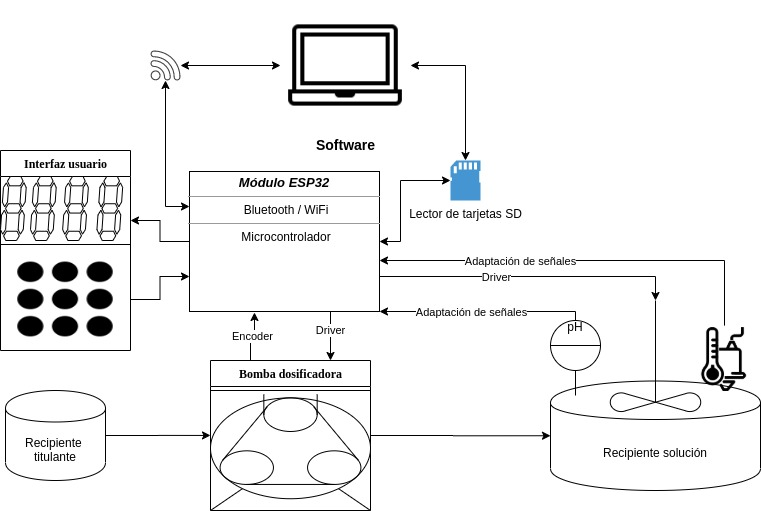
\includegraphics[width=1\textwidth]{./Figuras/diagBloques.jpg}
\caption{Diagrama en bloques del sistema}
\label{fig:diagBloques}
\end{figure}

%\vspace{25px}



\section{Identificación y análisis de los interesados}
\label{sec:interesados}

%Nota: (borrar esto y todas las consignas en color rojo antes de entregar este documento).
 
%Es inusual que una misma persona esté en más de un rol, incluso en proyectos chicos.
 
%Si se considera que una persona cumple dos o más roles, entonces sólo dejarla en el rol más importante. Por ejemplo:

%\begin{itemize}
%\item Si una persona es Cliente pero también colabora u orienta, dejarla solo como Cliente.
%\item Si una persona es el Responsable, no debe ser colocado también como Miembro del equipo.
%\end{itemize}

%Pero en cambio sí es usual que el Cliente y el Auspiciante sean el mismo, por ejemplo.

\begin{table}[ht]
%\caption{Identificación de los interesados}
%\label{tab:interesados}
\begin{tabularx}{\linewidth}{@{}|l|X|X|l|@{}}
\hline
\rowcolor[HTML]{C0C0C0} 
Rol           & Nombre y Apellido & Organización 	& Puesto 	\\ \hline
Cliente       & \clientename      &\empclientename	& Co-Directora de proyecto    	\\ \hline
%Impulsor      &        -          &      -        	&    -    	\\ \hline
Responsable   & \authorname       & FIUBA        	& Alumno 	\\ \hline
Colaborador & Leonardo Anchino  & GISAI - UTN    	& Becario      	\\ \hline
Colaborador & Lorenzo Depetris  & GISAI - UTN    	& Becario      	\\ \hline
Orientador    & \supname	      & \pertesupname 	& Director	Trabajo final \\ \hline
%Equipo        & % miembro1 \newline 
%						 -         &   -           	&  -      	\\ \hline
%Opositores    &      -            &   -           	&  -      	\\ \hline
Usuario final & Laboratorio de Servicios & UTN FRSCO & -        	\\ \hline
\end{tabularx}
\end{table}

%El Director suele ser uno de los Orientadores.
%No dejar celdas vacías; si no hay nada que poner en una celda colocar un signo ``-''.
%No dejar filas vacías; si no hay nada que poner en una fila entonces eliminarla.
%Sería deseable listar a continuación de la tabla las principales características de cada interesado.
 
%Por ejemplo:
%\begin{itemize}
%\item Auspiciante: es riguroso y exigente con la rendición de gastos. Tener mucho cuidado con esto.
%\item Equipo: Juan Perez, suele pedir licencia porque tiene un familiar con una enfermedad. Planificar considerando esto.
%\item Orientador: María Gómez, nos va a poder ayudar mucho con la gestión de impuestos.
%\end{itemize}

\section{1. Propósito del proyecto}
\label{sec:proposito}


El propósito de este proyecto es desarrollar el prototipo de un sistema embebido que permita automatizar y controlar el ensayo de titulación potenciométrica.


\section{2. Alcance del proyecto}
\label{sec:alcance}

El proyecto incluye:
\begin{itemize}
\item Una interfaz de usuario que permite la configuración y calibración del dispositivo, asi como también dar inicio al proceso de titulación.
\item La visualización de la curva de potencial respecto al volumen de titulante inyectado.
\item El control de la bomba que inyecta el titulante en la muestra
\item El cálculo y visualización del resultado de la titulación. El resultado es el volumen de titulante utilizado al momento de producirse un punto de inflexión en la curva.
\item El almacenamiento de los datos del ensayo en una memoria SD
\item La visualización de los datos del ensayo en una página web, a través de una conexión wifi local.
\end{itemize}

El proyecto no incluye:
\begin{itemize}
\item El manejo del dispositivo de manera remota.
\item El diseño de gabinetes u otras partes mecánicas. 
\end{itemize}

\section{3. Supuestos del proyecto}
\label{sec:supuestos}

Para el desarrollo del presente proyecto se supone que:

\begin{itemize}
\item El desarrollo de la bomba peristáltica y demás partes mécanicas estarán desarrolladas en el tiempo previsto.
\item El dinero disponible será suficiente para la adquisición de los materiales en el contexto macroeconómico actual
\item El aislamiento y/o distanciamento preventivo social y obligatorio no impidedirá la adquisición de materiales ni retrasará las pruebas y verificaciones del dispositivo.
\end{itemize}

\section{4. Requerimientos} %Los requerimientos deben numerarse y de ser posible agruparlos por afinidad:
\label{sec:requerimientos}

\begin{enumerate}
\item Grupo de requerimientos asociados con interfaces externas
	\begin{enumerate}
	\item El dispositivo deberá tener una pantalla táctil a través de la cual el usuario podrá interactuar con un menú de navegación.
	\item El menú deberá incluir una opción de configuración, una de calibración, una de titulación y otra de conexión.
	\item La opción de configuración deberá permitir elegir los valores de tres muestras patrones \textit{(buffers)} que se utilizarán en la calibración.
	\item La opción configuración deberá permitir elegir el volumen de corte de la titulación.
	\item La opción configuración deberá permitir elegir si utilizar o no el agitador.
	\item La opción calibración deberá permitir elegir con cual de los tres \textit{buffers} se calibrará y dar la opción de guardar el valor leído una vez realizada la medición. También debe dar la opción de cancelar sin guardar.
	\item La opción de titulación debe pedir al usuario que acepte el inicio del ensayo o regresar al menú principal. En caso de aceptar, debe mostrar el valor actual leído y una gráfica de pH en el eje de la ordenadas y de volumen de titulante añadido en el eje de las abcisas.
	\item La opción conexión debe mostrar los datos para que un dispositivo pueda conectarse a la red wifi del titulador. 
	\end{enumerate}
	
\item Grupo de requerimientos asociados con funciones
	\begin{enumerate}
	\item El sistema deberá ser capaz de leer y mostrar el potencial entregado por un electrodo de pH, con una resolución de 1 mV para la lectura del potencial y de 0,01 pH para su conversión a pH.
	\item El sistema deberá ser capaz de controlar la cantidad de pasos que realiza un motor paso a paso bipolar asociado a la bomba, asi como también el tiempo entre cada paso.
	\item Cada paso debe producir la inyección de titulante en la muestra en una cantidad máxima de 0,1 ml por paso.
	\item El tiempo mínimo de espera entre cada paso debe ser de 1 segundo luego que la lectura de potencial se haya estabilizado.
	\item El sistema deberá accionar el motor de la bomba en el momento que el usuario lo solicite y finalizar cuando se haya inyectado la cantidad de volumen indicada por el usuario como volumen de corte.
	\item Cuando el proceso de titulación comience, el agitador debe activarse si así lo indica el menú de configuración.
	\item Cada valor de volumen añadido junto al valor de potencial asocidado deberá guardarse en un memoria sd y mostrarse en un página web. No es necesario que esto se haga en tiempo real.
	\item Se deberá medir la temperatura para realizar ajustes en el valor de pH cuando la temperatura ambiente sea menor a 10 grados centígrados o mayor a 40 grados centígrados.
	\end{enumerate}
	
\item Grupo de requerimientos asociados con rendimiento y capacidad:
	\begin{enumerate}
	\item El sistema deberá ser capaz de realizar titulaciones que involucren una cantidad mínima de 50 ml de titulante y un cantidad máxima de 100 ml.
	\item El sistema deberá ser capaz de guardar en la memoria sd todos los datos generados en una titulación. Al iniciar otro proceso de titulación, los datos de la titulación anterior serán eliminados.
	\end{enumerate}
\end{enumerate}

\section{Historias de usuarios (\textit{Product backlog})}
\label{sec:backlog}

\begin{consigna}{red}
Descripción: En esta sección se deben incluir las historias de usuarios y su ponderación (\textit{history points}). Recordar que las historias de usuarios son descripciones cortas y simples de una característica contada desde la perspectiva de la persona que desea la nueva capacidad, generalmente un usuario o cliente del sistema.

La ponderación es un número entero que representa el tamaño de la historia comparada con otras historias de similar tipo.
\end{consigna}


\section{5. Entregables principales del proyecto}
\label{sec:entregables}

\begin{itemize}
\item Prototipo funcional
\item Manual de uso
\item Diagrama esquemático
\item Código fuente
\item Memoria técnica
\end{itemize}

\section{6. Desglose del trabajo en tareas}
\label{sec:wbs}

\begin{enumerate}
\item Investigación y documentación (60 hs)
	\begin{enumerate}
	\item Analizar diferentes procesos de titulación y tituladores del mercado (10 hs)
	\item Seleccionar los componetes adecuados con sus respectivas hojas de datos(10 hs)
	\item Analizar el funcionamiento de los compontentes (40 hs)
	\end{enumerate}
\item Diseño general (50 hs)
	\begin{enumerate}
	\item Diseño de diagrama de módulos (10 hs)
	\item Diseño de diagramas de flujo (10 hs)
	\item Diseño de diagrama de conexiones (10 hs)
	\item Diseño de esquemático y pcb (20 hs)
	\end{enumerate}
\item Desarrollo del hardware (20 hs)
	\begin{enumerate}
	\item Construcción del prototipo del pcb (15 hs)
	\item Conexión de los diferentes componetes (5 hs)
	\end{enumerate}
\item Desarrollo del firmware (280 hs)	
	\begin{enumerate}
	\item Desarrollo del menú de usuario mediante pantalla táctil (40 hs)
	\item Desarrollo del módulo de calibración (40 hs)
	\item Desarrollo del módulo de medición (40 hs)
	\item Desarrollo del módulo de control de la bomba (40 hs)
	\item Desarrollo del módulo de guardado de datos en sd (40 hs)
	\item Desarrollo del módulo de conexión wifi y página web (40 hs)
	\item Desarrollo del módulo de calculo del volumen en el punto de inflexión (40 hs)
	\end{enumerate}
\item Calibración y puesta en funcionamiento (50 hs)
	\begin{enumerate}	
	\item Calibración del módulo de medición de pH (25 hs)
	\item Calibración del módulo de control de la bomba (20 hs)
	\item Puesta en funcionamiento  (5 hs)
	\end{enumerate}
\item Testing (100hs)
	\begin{enumerate}	
	\item Test de cada módulo de software (40 hs)
	\item Ensayos del sistema completo con diferentes tipos de titulaciones (40 hs)
	\item Correción de errores (20 hs)
	\end{enumerate}
\item Presentación del trabajo (80 hs)
	\begin{enumerate}
	\item Redacción de la memoria escrita (60 hs)
	\item Preparación de la presentación pública del trabajo (20 hs)	
	\end{enumerate}
\end{enumerate}

Cantidad total de horas: (640 hs)

\section{7. Diagrama de Activity On Node}
\label{sec:AoN}
%La figura \ref{fig:AoN} fue elaborada con el paquete latex tikz y pueden consultar la siguiente referencia \textit{online}:
%\url{https://www.overleaf.com/learn/latex/LaTeX_Graphics_using_TikZ:_A_Tutorial_for_Beginners_(Part_3)\%E2\%80\%94Creating_Flowcharts}
En la Figura 2 se muestra el diagrama de Activity on Node del proyecto. Se observa que la línea remarcada indica el camino crítico del proyecto, con un total de 620 horas.

\begin{figure}[htpb]
\centering 
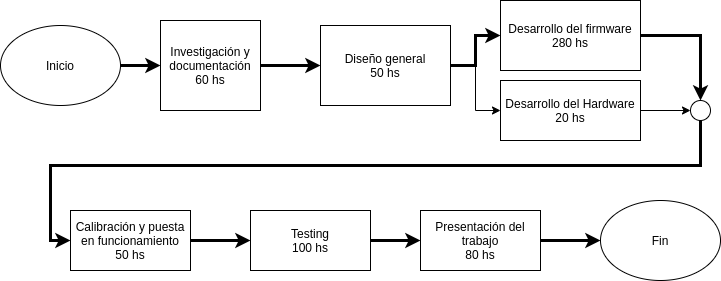
\includegraphics[width=1\textwidth]{./Figuras/AoN.png}
\caption{Diagrama en \textit{Activity on Node}}
\label{fig:AoN}
\end{figure}



\section{8. Diagrama de Gantt}
\label{sec:gantt}


\begin{figure}[p]
\centering 
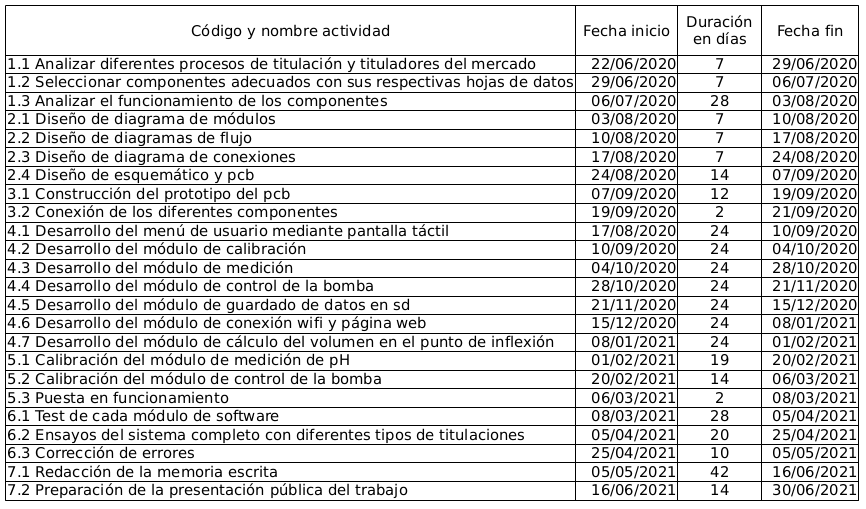
\includegraphics[width=1\textwidth]{./Figuras/TablaGantt.png}
\caption{Diagrama de Gantt: Tabla}
\label{fig:tablaGantt}
\end{figure}

\begin{figure}[p]

\centering 
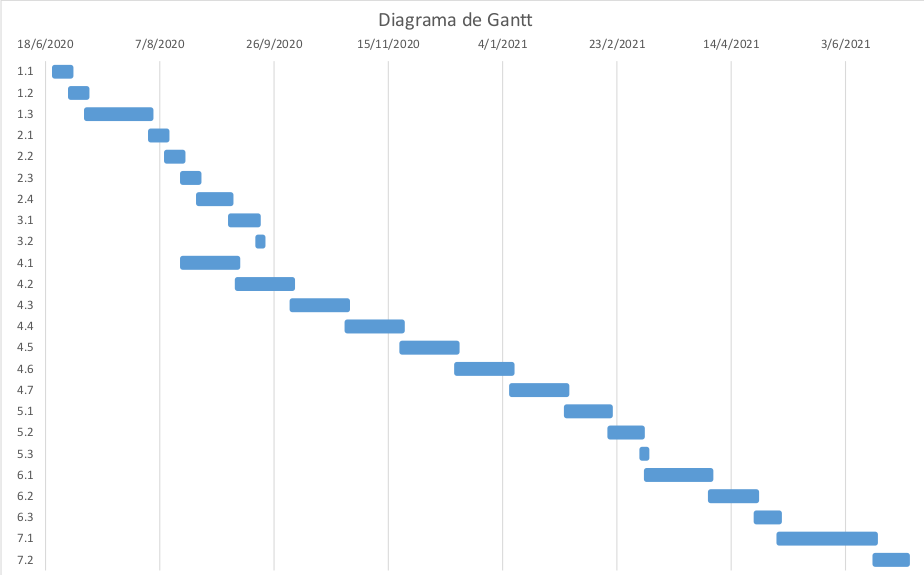
\includegraphics[width=1\textwidth]{./Figuras/DiagramaGantt.png}
\caption{Diagrama de Gantt: Gráfico}
\label{fig:diagramaGantt}
\end{figure}

\section{9. Matriz de uso de recursos de materiales}
\label{sec:recursos}

\begin{table}[h]
\label{tab:recursos}
\centering
\begin{tabularx}{\linewidth}{@{}|c|X|X|X|X|X|X|X|@{}}
\hline
\cellcolor[HTML]{C0C0C0} & \cellcolor[HTML]{C0C0C0} & \multicolumn{6}{c|}{\cellcolor[HTML]{C0C0C0}Recursos requeridos (horas)} \\ \cline{3-8} 
\multirow{-2}{*}{\cellcolor[HTML]{C0C0C0}\begin{tabular}[c]{@{}c@{}}Código\\ WBS\end{tabular}} & \multirow{-2}{*}{\cellcolor[HTML]{C0C0C0}\begin{tabular}[c]{@{}c@{}}Nombre \\ tarea\end{tabular}} & PC & Módulo pantalla  & Electrodo  & Bomba    & SD   & Insumos varios\\ \hline
1& Investigación y documentación   &60  &  &  &&  &\\ \hline
2& Diseño general  &50  &  &  &&  &\\ \hline
3& Desarrollo de hardware &  &  &  & & &20\\ \hline
4& Desarrollo del firmware   &280  &  &  & & &\\ \hline
5& Calibración y puesta en funcionamiento  &5  &60  &30  &25 &5 &\\ \hline
6& Testing 	 &100  &100  &100  &100 &100 &\\ \hline
7&Presentación del trabajo   &80  &  &  & & &\\ \hline
\end{tabularx}%
\end{table}


\section{10. Presupuesto detallado del proyecto}
\label{sec:presupuesto}


\begin{table}[htpb]
\centering
\begin{tabularx}{\linewidth}{@{}|X|c|r|r|@{}}
\hline
\rowcolor[HTML]{C0C0C0} 
\multicolumn{4}{|c|}{\cellcolor[HTML]{C0C0C0}COSTOS DIRECTOS} \\ \hline
\rowcolor[HTML]{C0C0C0} 
Descripción &
  \multicolumn{1}{c|}{\cellcolor[HTML]{C0C0C0}Cantidad} &
  \multicolumn{1}{c|}{\cellcolor[HTML]{C0C0C0}Valor unitario} &
  \multicolumn{1}{c|}{\cellcolor[HTML]{C0C0C0}Valor total} \\ \hline
 ESP32&
  \multicolumn{1}{c|}{1} &
  \multicolumn{1}{c|}{\$1400} &
  \multicolumn{1}{c|}{\$1400} \\ \hline
 Display táctil con lector SD&
  \multicolumn{1}{c|}{1} &
  \multicolumn{1}{c|}{\$1300} &
  \multicolumn{1}{c|}{\$1300} \\ \hline
Driver drv8825&
  \multicolumn{1}{c|}{2} &
  \multicolumn{1}{c|}{\$400} &
  \multicolumn{1}{c|}{\$800} \\ \hline
Modulo Ph-4502c&
  \multicolumn{1}{c|}{1} &
  \multicolumn{1}{c|}{\$4000} &
  \multicolumn{1}{c|}{\$4000} \\ \hline
Modulo Ph-4502c&
  \multicolumn{1}{c|}{1} &
  \multicolumn{1}{c|}{\$4000} &
  \multicolumn{1}{c|}{\$4000} \\ \hline
PCB&
  \multicolumn{1}{c|}{1} &
  \multicolumn{1}{c|}{\$500} &
  \multicolumn{1}{c|}{\$500} \\ \hline
\multicolumn{3}{|c|}{SUBTOTAL} &
  \multicolumn{1}{c|}{\$12000} \\ \hline
\rowcolor[HTML]{C0C0C0} 
\multicolumn{4}{|c|}{\cellcolor[HTML]{C0C0C0}COSTOS INDIRECTOS} \\ \hline
\rowcolor[HTML]{C0C0C0} 
Descripción &
  \multicolumn{1}{c|}{\cellcolor[HTML]{C0C0C0}Cantidad} &
  \multicolumn{1}{c|}{\cellcolor[HTML]{C0C0C0}Valor unitario} &
  \multicolumn{1}{c|}{\cellcolor[HTML]{C0C0C0}Valor total} \\ \hline
Insumos varios&
  \multicolumn{1}{c|}{1} &
  \multicolumn{1}{c|}{\$3000} &
  \multicolumn{1}{c|}{\$3000} \\ \hline

\multicolumn{3}{|c|}{SUBTOTAL} &
  \multicolumn{1}{c|}{3000} \\ \hline
\rowcolor[HTML]{C0C0C0}
\multicolumn{3}{|c|}{TOTAL} &\$15000
   \\ \hline
\end{tabularx}%
\end{table}


\section{11. Matriz de asignación de responsabilidades}
\label{sec:responsabilidades}

\begin{table}[htpb]

\centering
\resizebox{\textwidth}{!}{%
\begin{tabular}{|c|c|c|c|c|c|}
\hline
\rowcolor[HTML]{C0C0C0} 
\cellcolor[HTML]{C0C0C0} &
  \cellcolor[HTML]{C0C0C0} &
  \multicolumn{4}{c|}{\cellcolor[HTML]{C0C0C0}Listar todos los nombres y roles del proyecto} \\ \cline{3-6} 
\rowcolor[HTML]{C0C0C0} 
\cellcolor[HTML]{C0C0C0} &
  \cellcolor[HTML]{C0C0C0} &
  Responsable &
  Director &
  Colaboradores &
  Cliente \\ \cline{3-6} 
\rowcolor[HTML]{C0C0C0} 
\multirow{-3}{*}{\cellcolor[HTML]{C0C0C0}\begin{tabular}[c]{@{}c@{}}Código\\ WBS\end{tabular}} &
  \multirow{-3}{*}{\cellcolor[HTML]{C0C0C0}Nombre de la tarea} &
  \authorname &
  \supname &
  Anchino y Depetris &
  \clientename \\ \hline
1& Investigación y documentación   &P  &C & &C  \\ \hline
2& Diseño general  &P  &I &C &A  \\ \hline
3& Desarrollo de hardware &P  &  &C  & \\ \hline
4& Desarrollo del firmware   &P  &I &C &  \\ \hline
5& Calibración y puesta en funcionamiento  &P  &I &S &I  \\ \hline
6& Testing 	 &P  & & &I  \\ \hline
7&Presentación del trabajo   &P  &A & &  \\ \hline
\end{tabular}%
}
\end{table}

{\footnotesize
Referencias:
\begin{itemize}
	\item P = Responsabilidad Primaria
	\item S = Responsabilidad Secundaria
	\item A = Aprobación
	\item I = Informado
	\item C = Consultado
\end{itemize}
} %footnotesize


\section{12. Gestión de riesgos}
\label{sec:riesgos}

\begin{consigna}{red}
a) Identificación de los riesgos (al menos cinco) y estimación de sus consecuencias:
 
Riesgo 1: detallar el riesgo (riesgo es algo que si ocurre altera los planes previstos)
\begin{itemize}
\item Severidad (S): mientras más severo, más alto es el número (usar números del 1 al 10).\\
Justificar el motivo por el cual se asigna determinado número de severidad (S).
\item Probabilidad de ocurrencia (O): mientras más probable, más alto es el número (usar del 1 al 10).\\
Justificar el motivo por el cual se asigna determinado número de (O). 
\end{itemize}   

Riesgo 2:
\begin{itemize}
\item Severidad (S): 
\item Ocurrencia (O):
\end{itemize}

Riesgo 3:
\begin{itemize}
\item Severidad (S): 
\item Ocurrencia (O):
\end{itemize}


b) Tabla de gestión de riesgos:      (El RPN se calcula como RPN=SxO)

\begin{table}[htpb]
\centering
\begin{tabularx}{\linewidth}{@{}|X|c|c|c|c|c|c|@{}}
\hline
\rowcolor[HTML]{C0C0C0} 
Riesgo & S & O & RPN & S* & O* & RPN* \\ \hline
       &   &   &     &    &    &      \\ \hline
       &   &   &     &    &    &      \\ \hline
       &   &   &     &    &    &      \\ \hline
       &   &   &     &    &    &      \\ \hline
       &   &   &     &    &    &      \\ \hline
\end{tabularx}%
\end{table}

Criterio adoptado: 
Se tomarán medidas de mitigación en los riesgos cuyos números de RPN sean mayores a ....

Nota: los valores marcados con (*) en la tabla corresponden luego de haber aplicado la mitigación.

c) Plan de mitigación de los riesgos que originalmente excedían el RPN máximo establecido:
 
Riesgo 1: Plan de mitigación (si por el RPN fuera necesario elaborar un plan de mitigación).
  Nueva asignación de S y O, con su respectiva justificación:
  - Severidad (S): mientras más severo, más alto es el número (usar números del 1 al 10).
          Justificar el motivo por el cual se asigna determinado número de severidad (S).
  - Probabilidad de ocurrencia (O): mientras más probable, más alto es el número (usar del 1 al 10).
          Justificar el motivo por el cual se asigna determinado número de (O).

Riesgo 2: Plan de mitigación (si por el RPN fuera necesario elaborar un plan de mitigación).
 
Riesgo 3: Plan de mitigación (si por el RPN fuera necesario elaborar un plan de mitigación)

\end{consigna}


\section{13. Gestión de la calidad}
\label{sec:calidad}

\begin{consigna}{red}
Para cada uno de los requerimientos del proyecto indique:
\begin{itemize} 
\item Req \#1: Copiar acá el requerimiento.

Verificación y validación:

\begin{itemize}
\item Verificación para confirmar si se cumplió con lo requerido antes de mostrar el sistema al cliente:\\
Detallar 
\item Validación con el cliente para confirmar que está de acuerdo en que se cumplió con lo requerido:\\
Detallar  
\end{itemize}

\end{itemize}

Tener en cuenta que en este contexto se pueden mencionar simulaciones, cálculos, revisión de hojas de datos, consulta con expertos, etc.

\end{consigna}

\section{14. Comunicación del proyecto}
\label{sec:comunicaciones}

\begin{consigna}{red}
El plan de comunicación del proyecto es el siguiente:
\end{consigna}

% Please add the following required packages to your document preamble:
% \usepackage{graphicx}
% \usepackage[table,xcdraw]{xcolor}
% If you use beamer only pass "xcolor=table" option, i.e. \documentclass[xcolor=table]{beamer}
\begin{table}[htpb]
\centering
\resizebox{\textwidth}{!}{%
\begin{tabular}{|c|c|c|c|c|c|}
\hline
\rowcolor[HTML]{C0C0C0} 
\multicolumn{6}{|c|}{\cellcolor[HTML]{C0C0C0}PLAN DE COMUNICACIÓN DEL PROYECTO}           \\ \hline
\rowcolor[HTML]{C0C0C0} 
¿Qué comunicar? & Audiencia & Propósito & Frecuencia & Método de comunicac. & Responsable \\ \hline
                &           &           &            &                      &             \\ \hline
                &           &           &            &                      &             \\ \hline
                &           &           &            &                      &             \\ \hline
                &           &           &            &                      &             \\ \hline
                &           &           &            &                      &             \\ \hline
\end{tabular}%
}
\end{table}

\section{15. Gestión de Compras}
\label{sec:compras}

\begin{consigna}{red}
En caso de tener que comprar elementos o contratar servicios:
a) Explique con qué criterios elegiría a un proveedor.
b) Redacte el Statement of Work correspondiente.
\end{consigna}

\section{16. Seguimiento y control}
\label{sec:seguimiento}

\begin{consigna}{red}
Para cada tarea del proyecto establecer la frecuencia y los indicadores con los se seguirá su avance y quién será el responsable de hacer dicho seguimiento y a quién debe comunicarse la situación (en concordancia con el Plan de Comunicación del proyecto).

El indicador de avance tiene que ser algo medible, mejor incluso si se puede medir en \% de avance. Por ejemplo,se pueden indicar en esta columna cosas como ``cantidad de conexiones ruteadeas'' o ``cantidad de funciones implementadas'', pero no algo genérico y ambiguo como ``\%'', porque el lector no sabe porcentaje de qué cosa.

\end{consigna}

\begin{table}[!htpb]
\centering
\begin{tabularx}{\linewidth}{@{}|X|X|X|X|X|X|@{}}
\hline
\rowcolor[HTML]{C0C0C0} 
\multicolumn{6}{|c|}{\cellcolor[HTML]{C0C0C0}SEGUIMIENTO DE AVANCE}                                                                       \\ \hline
\rowcolor[HTML]{C0C0C0} 
Tarea del WBS & Indicador de avance & Frecuencia de reporte & Resp. de seguimiento & Persona a ser informada & Método de comunic. \\ \hline
 &  &  &  &  &  \\ \hline
 &  &  &  &  &  \\ \hline
 &  &  &  &  &  \\ \hline
 &  &  &  &  &  \\ \hline
 &  &  &  &  &  \\ \hline
\end{tabularx}%
%}
\end{table}

\section{17. Procesos de cierre}    
\label{sec:cierre}

\begin{consigna}{red}
Establecer las pautas de trabajo para realizar una reunión final de evaluación del proyecto, tal que contemple las siguientes actividades:

\begin{itemize}
\item Pautas de trabajo que se seguirán para analizar si se respetó el Plan de Proyecto original:
 - Indicar quién se ocupará de hacer esto y cuál será el procedimiento a aplicar. 
\item Identificación de las técnicas y procedimientos útiles e inútiles que se utilizaron, y los problemas que surgieron y cómo se solucionaron:
 - Indicar quién se ocupará de hacer esto y cuál será el procedimiento para dejar registro.
\item Indicar quién organizará el acto de agradecimiento a todos los interesados, y en especial al equipo de trabajo y colaboradores:
  - Indicar esto y quién financiará los gastos correspondientes.
\end{itemize}

\end{consigna}


\end{document}
